\documentclass{article}

% content/resources/templates/preamble.tex
\usepackage[margin=0.6in]{geometry}
\author{Milav Dabgar}
\usepackage{amsmath,amssymb,amsthm}
\usepackage{booktabs}
\usepackage{multirow}
\usepackage{xcolor}
\usepackage{tcolorbox}
\tcbuselibrary{breakable,skins}
\usepackage[colorlinks=true,linkcolor=blue]{hyperref}
\usepackage{titlesec}
\usepackage{enumitem}
\usepackage{tikz}
\usepackage{pgfplots}
\usepackage{circuitikz}
\usepackage[version=4]{mhchem}
\usepackage{longtable}
\usepackage{array}
\usepackage{float}
\usepackage{caption}
\usepackage{listings}

\lstset{
  basicstyle=\small\ttfamily,
  breaklines=true,
  breakatwhitespace=false,
  postbreak=\mbox{\textcolor{red}{$\hookrightarrow$}\space},
  float=false,
  numbers=left,
  numberstyle=\tiny\color{gray},
  numbersep=10pt,
  xleftmargin=2em,
  keywordstyle=\color{blue},
  commentstyle=\color{green!60!black},
  stringstyle=\color{purple},
  backgroundcolor=\color{gray!5},
  showstringspaces=false,
  tabsize=2,
  captionpos=b,
  keepspaces=true,
  columns=flexible
}

\pgfplotsset{compat=1.18}
\usetikzlibrary{shapes,arrows,positioning,calc,patterns,decorations.pathmorphing,decorations.markings,arrows.meta}

% Color scheme
\definecolor{headcolor}{RGB}{0,102,204}
\definecolor{keycolor}{RGB}{220,20,60}
\definecolor{solutioncolor}{RGB}{34,139,34}
\definecolor{mnemoniccolor}{RGB}{148,0,211}
\definecolor{codecolor}{RGB}{0,0,100}

% Spacing
\setlength{\parskip}{3pt}
\setlist[itemize]{nosep}
\setlist[enumerate]{nosep}

% Title formatting
\titleformat{\section}{\Large\bfseries\color{headcolor}}{\thesection}{1em}{}
\titleformat{\subsection}{\large\bfseries\color{headcolor}}{\thesubsection}{1em}{}

% Pandoc tightlist compatibility
\providecommand{\tightlist}{%
  \setlength{\itemsep}{0pt}\setlength{\parskip}{0pt}}

% Pandoc longtable compatibility
\newcounter{none}
\def\thenone{}


% content/resources/templates/english-boxes.tex

% Custom environments
\newtcolorbox{solutionbox}{
 breakable,
 enhanced,
 colback=solutioncolor!5!white,
 colframe=solutioncolor!75!black,
 fonttitle=\bfseries,
 title=Solution
}

\newtcolorbox{solutionboxnobreak}{
 colback=solutioncolor!5!white,
 colframe=solutioncolor!75!black,
 fonttitle=\bfseries,
 title=Solution
}

\newtcolorbox{keyformula}{
 breakable,
 enhanced,
 colback=keycolor!5!white,
 colframe=keycolor!75!black,
 fonttitle=\bfseries,
 title=Key Formula
}

\newtcolorbox{mnemonicboxenv}{
 breakable,
 enhanced,
 colback=mnemoniccolor!5!white,
 colframe=mnemoniccolor!75!black,
 fonttitle=\bfseries,
 title=Mnemonic
}

\newcommand{\mnemonicbox}[1]{%
  \begin{mnemonicboxenv}
    #1
  \end{mnemonicboxenv}
}


% Custom commands for GTU solutions
% This file defines semantic commands for consistent formatting

% Question command with automatic formatting
\newcommand{\question}[2]{%
  \section*{Question #1}%
  \textbf{#2}%
}

% OR question variant
\newcommand{\questionor}[2]{%
  \section*{Question #1 OR}%
  \textbf{#2}%
}

% Proper table environment with caption
\newenvironment{answertable}[1]{%
  \begin{table}[htbp]
  \centering
  \caption{#1}
}{%
  \end{table}
}

% Proper figure environment for diagrams
\newenvironment{answerdiagram}[1]{%
  \begin{figure}[htbp]
  \centering
  \caption{#1}
}{%
  \end{figure}
}

% Semantic markup for key terms
\newcommand{\keyword}[1]{\textbf{#1}}
\newcommand{\code}[1]{\texttt{#1}}
\newcommand{\classname}[1]{\texttt{#1}}
\newcommand{\methodname}[1]{\texttt{#1}}

% Proper quotation marks
\newcommand{\mnemonic}[1]{``#1''}


\title{Foundation of AI and ML (4351601) - Summer 2024 Solution}
\date{May 16, 2024}

\begin{document}
\maketitle

\questionmarks{1(a)}{3}{What do you mean by Narrow AI or Weak AI?}
\begin{solutionbox}
\textbf{Narrow AI} or \textbf{Weak AI} refers to artificial intelligence systems designed to perform specific, limited tasks within a narrow domain.

\begin{center}
\captionof{table}{Narrow AI Characteristics}
\begin{tabulary}{\linewidth}{L L}
\hline
\textbf{Aspect} & \textbf{Description} \\
\hline
\textbf{Scope} & Limited to specific tasks \\
\textbf{Intelligence} & Task-specific expertise \\
\textbf{Examples} & Siri, chess programs, recommendation systems \\
\textbf{Learning} & Pattern recognition within domain \\
\hline
\end{tabulary}
\end{center}
\end{solutionbox}

\begin{mnemonicbox}
\mnemonic{Narrow = Specific Tasks Only}
\end{mnemonicbox}

\questionmarks{1(b)}{4}{Define: Classification, Regression, Clustering, Association Analysis.}
\begin{solutionbox}
\begin{center}
\captionof{table}{Machine Learning Techniques}
\begin{tabulary}{\linewidth}{L L L L}
\hline
\textbf{Technique} & \textbf{Definition} & \textbf{Type} & \textbf{Example} \\
\hline
\textbf{Classification} & Predicts discrete categories/classes & Supervised & Email spam detection \\
\textbf{Regression} & Predicts continuous numerical values & Supervised & House price prediction \\
\textbf{Clustering} & Groups similar data points & Unsupervised & Customer segmentation \\
\textbf{Association Analysis} & Finds relationships between variables & Unsupervised & Market basket analysis \\
\hline
\end{tabulary}
\end{center}
\end{solutionbox}

\begin{mnemonicbox}
\mnemonic{CRCA - Categories, Real-numbers, Clusters, Associations}
\end{mnemonicbox}

\questionmarks{1(c)}{7}{Illuminate the three main components of neuron.}
\begin{solutionbox}
The three main components of a biological neuron that inspire artificial neural networks are:

\begin{center}
\begin{tikzpicture}[node distance=1.5cm, auto]
    \node [gtu block] (Dendrites) {Dendrites};
    \node [gtu block, right=of Dendrites] (Soma) {Cell Body (Soma)};
    \node [gtu block, right=of Soma] (Axon) {Axon};
    \node [gtu state, below=0.5cm of Dendrites] {Input\\Receivers};
    \node [gtu state, below=0.5cm of Soma] {Processing\\Unit};
    \node [gtu state, below=0.5cm of Axon] {Output\\Transmitter};
    
    \path [gtu arrow] (Dendrites) -- node[above] {Signals} (Soma);
    \path [gtu arrow] (Soma) -- node[above] {Impulses} (Axon);
\end{tikzpicture}
\captionof{figure}{Neuron Components}
\end{center}

\begin{center}
\captionof{table}{Neuron Components}
\begin{tabulary}{\linewidth}{L L L}
\hline
\textbf{Component} & \textbf{Function} & \textbf{AI Equivalent} \\
\hline
\textbf{Dendrites} & Receive input signals from other neurons & Input layer/weights \\
\textbf{Cell Body (Soma)} & Processes and integrates signals & Activation function \\
\textbf{Axon} & Transmits output signals to other neurons & Output connections \\
\hline
\end{tabulary}
\end{center}

\textbf{Key Points:}
\begin{itemize}
    \item \textbf{Dendrites}: Act as input receivers with varying connection strengths.
    \item \textbf{Cell Body}: Sums inputs and applies threshold function.
    \item \textbf{Axon}: Carries processed signal to next neurons.
\end{itemize}
\end{solutionbox}

\begin{mnemonicbox}
\mnemonic{DCA - Dendrites Collect, Cell-body Calculates, Axon Announces}
\end{mnemonicbox}

\questionmarks{1(c) OR}{7}{Explicate back propagation method in Artificial Neural Network.}
\begin{solutionbox}
\textbf{Back Propagation} is a supervised learning algorithm used to train multi-layer neural networks by minimizing error through gradient descent.

\begin{center}
\begin{tikzpicture}[node distance=1.5cm, auto]
    \node [gtu block] (Forward) {Forward Pass};
    \node [gtu block, right=of Forward] (Output) {Calculate Output};
    \node [gtu block, below=1cm of Output] (Error) {Calculate Error};
    \node [gtu block, left=of Error] (Backward) {Backward Pass};
    \node [gtu block, below=1cm of Backward] (Gradient) {Calculate Gradients};
    \node [gtu block, right=of Gradient] (Update) {Update Weights};
    \node [gtu decision, below=1cm of Update] (Check) {Error Acceptable?};
    \node [gtu state, right=of Check] (Done) {Training Complete};
    
    \path [gtu arrow] (Forward) -- (Output);
    \path [gtu arrow] (Output) -- (Error);
    \path [gtu arrow] (Error) -- (Backward);
    \path [gtu arrow] (Backward) -- (Gradient);
    \path [gtu arrow] (Gradient) -- (Update);
    \path [gtu arrow] (Update) -- (Check);
    \path [gtu arrow] (Check) -- node[above] {Yes} (Done);
    \path [gtu arrow] (Check.west) -- node[above] {No} ++(-1.5,0) |- (Forward.west);
\end{tikzpicture}
\captionof{figure}{Back Propagation Flow}
\end{center}

\begin{center}
\captionof{table}{Back Propagation Steps}
\begin{tabulary}{\linewidth}{L L L}
\hline
\textbf{Step} & \textbf{Process} & \textbf{Formula} \\
\hline
\textbf{Forward Pass} & Calculate outputs layer by layer & \(y = f(\Sigma(w_i x_i + b))\) \\
\textbf{Error Calculation} & Compute loss function & \(E = \frac{1}{2}(target - output)^2\) \\
\textbf{Backward Pass} & Calculate error gradients & \(\delta = \partial E/\partial w\) \\
\textbf{Weight Update} & Adjust weights using learning rate & \(w_{new} = w_{old} - \eta \cdot \delta\) \\
\hline
\end{tabulary}
\end{center}

\textbf{Key Features:}
\begin{itemize}
    \item \textbf{Gradient Descent}: Uses calculus to find minimum error.
    \item \textbf{Chain Rule}: Propagates error backward through layers.
    \item \textbf{Learning Rate}: Controls speed of weight updates.
\end{itemize}
\end{solutionbox}

\begin{mnemonicbox}
\mnemonic{FEBU - Forward, Error, Backward, Update}
\end{mnemonicbox}

\questionmarks{2(a)}{3}{List out any five popular algorithms used in Machine Learning.}
\begin{solutionbox}
\begin{center}
\captionof{table}{Popular ML Algorithms}
\begin{tabulary}{\linewidth}{L L L}
\hline
\textbf{Algorithm} & \textbf{Type} & \textbf{Application} \\
\hline
\textbf{Linear Regression} & Supervised & Prediction of continuous values \\
\textbf{Decision Tree} & Supervised & Classification and regression \\
\textbf{K-Means Clustering} & Unsupervised & Data grouping \\
\textbf{Support Vector Machine} & Supervised & Classification with margins \\
\textbf{Random Forest} & Supervised & Ensemble learning \\
\hline
\end{tabulary}
\end{center}
\end{solutionbox}

\begin{mnemonicbox}
\mnemonic{LDKSR - Learn Data, Keep Samples, Run}
\end{mnemonicbox}

\questionmarks{2(b)}{4}{What is Expert System? List out its limitations and applications.}
\begin{solutionbox}
\textbf{Expert System} is an AI program that mimics human expert knowledge to solve complex problems in specific domains.

\begin{center}
\captionof{table}{Expert System Overview}
\begin{tabulary}{\linewidth}{L L}
\hline
\textbf{Aspect} & \textbf{Details} \\
\hline
\textbf{Definition} & AI system with domain-specific expertise \\
\textbf{Components} & Knowledge base, inference engine, user interface \\
\hline
\end{tabulary}
\end{center}

\textbf{Applications:}
\begin{itemize}
    \item \textbf{Medical Diagnosis}: Disease identification systems.
    \item \textbf{Financial Planning}: Investment advisory systems.
    \item \textbf{Fault Diagnosis}: Equipment troubleshooting.
\end{itemize}

\textbf{Limitations:}
\begin{itemize}
    \item \textbf{Limited Domain}: Works only in specific areas.
    \item \textbf{Knowledge Acquisition}: Difficult to extract expert knowledge.
    \item \textbf{Maintenance}: Hard to update and modify rules.
\end{itemize}
\end{solutionbox}

\begin{mnemonicbox}
\mnemonic{EXPERT - Explains Problems, Executes Rules, Tests}
\end{mnemonicbox}

\questionmarks{2(c)}{7}{What is tokenization? Explain with suitable example.}
\begin{solutionbox}
\textbf{Tokenization} is the process of breaking down text into smaller units called tokens (words, phrases, symbols) for NLP processing.

\begin{center}
\captionof{table}{Tokenization Types}
\begin{tabulary}{\linewidth}{L L L}
\hline
\textbf{Type} & \textbf{Description} & \textbf{Example} \\
\hline
\textbf{Word Tokenization} & Split by words & "Hello world" $\to$ ["Hello", "world"] \\
\textbf{Sentence Tokenization} & Split by sentences & "Hi. How are you?" $\to$ ["Hi.", "How are you?"] \\
\textbf{Subword Tokenization} & Split into subwords & "unhappy" $\to$ ["un", "happy"] \\
\hline
\end{tabulary}
\end{center}

\textbf{Code Example:}
\begin{lstlisting}[language=python]
import nltk
text = "Natural Language Processing is amazing!"
tokens = nltk.word_tokenize(text)
# Output: ['Natural', 'Language', 'Processing', 'is', 'amazing', '!']
\end{lstlisting}

\begin{center}
\begin{tikzpicture}[node distance=1.5cm, auto]
    \node [gtu block] (Raw) {Raw Text};
    \node [gtu block, right=of Raw] (Token) {Tokenization};
    \node [gtu block, right=of Token] (Clean) {Clean Tokens};
    \node [gtu block, right=of Clean] (Process) {Further Processing};
    
    \path [gtu arrow] (Raw) -- (Token);
    \path [gtu arrow] (Token) -- (Clean);
    \path [gtu arrow] (Clean) -- (Process);
\end{tikzpicture}
\captionof{figure}{Tokenization Process}
\end{center}

\textbf{Key Benefits:}
\begin{itemize}
    \item \textbf{Standardization}: Converts text to uniform format.
    \item \textbf{Analysis Ready}: Prepares text for ML algorithms.
    \item \textbf{Feature Extraction}: Enables statistical analysis.
\end{itemize}
\end{solutionbox}

\begin{mnemonicbox}
\mnemonic{TOKEN - Text Operations Keep Everything Normalized}
\end{mnemonicbox}

\questionmarks{2(a) OR}{3}{Compare Supervised and Unsupervised Learning.}
\begin{solutionbox}
\begin{center}
\captionof{table}{Supervised vs Unsupervised Learning}
\begin{tabulary}{\linewidth}{L L L}
\hline
\textbf{Aspect} & \textbf{Supervised Learning} & \textbf{Unsupervised Learning} \\
\hline
\textbf{Training Data} & Labeled data with target outputs & Unlabeled data without targets \\
\textbf{Goal} & Predict specific outcomes & Discover hidden patterns \\
\textbf{Examples} & Classification, Regression & Clustering, Association rules \\
\textbf{Evaluation} & Accuracy, precision, recall & Silhouette score, elbow method \\
\textbf{Applications} & Email spam, price prediction & Customer segmentation, anomaly detection \\
\hline
\end{tabulary}
\end{center}
\end{solutionbox}

\begin{mnemonicbox}
\mnemonic{SU - Supervised Uses labels, Unsupervised Uncovers patterns}
\end{mnemonicbox}

\questionmarks{2(b) OR}{4}{Explain all about AI applications in Healthcare, Finance and Manufacturing.}
\begin{solutionbox}
\begin{center}
\captionof{table}{AI Applications by Industry}
\begin{tabulary}{\linewidth}{L L L}
\hline
\textbf{Industry} & \textbf{Applications} & \textbf{Benefits} \\
\hline
\textbf{Healthcare} & Medical imaging, drug discovery, diagnosis & Improved accuracy, faster treatment \\
\textbf{Finance} & Fraud detection, algorithmic trading, credit scoring & Risk reduction, automated decisions \\
\textbf{Manufacturing} & Quality control, predictive maintenance, robotics & Efficiency, cost reduction \\
\hline
\end{tabulary}
\end{center}

\textbf{Healthcare Examples:}
\begin{itemize}
    \item \textbf{Medical Imaging}: AI detects cancer in X-rays and MRIs.
    \item \textbf{Drug Discovery}: AI accelerates new medicine development.
\end{itemize}

\textbf{Finance Examples:}
\begin{itemize}
    \item \textbf{Fraud Detection}: Real-time transaction monitoring.
    \item \textbf{Robo-advisors}: Automated investment management.
\end{itemize}

\textbf{Manufacturing Examples:}
\begin{itemize}
    \item \textbf{Quality Control}: Automated defect detection.
    \item \textbf{Predictive Maintenance}: Equipment failure prediction.
\end{itemize}
\end{solutionbox}

\begin{mnemonicbox}
\mnemonic{HFM - Health, Finance, Manufacturing benefit from AI}
\end{mnemonicbox}

\questionmarks{2(c) OR}{7}{What is syntactic analysis and how it is differ from lexical analysis?}
\begin{solutionbox}
\textbf{Syntactic Analysis} examines the grammatical structure of sentences, while \textbf{Lexical Analysis} breaks text into meaningful tokens.

\begin{center}
\captionof{table}{Lexical vs Syntactic Analysis}
\begin{tabulary}{\linewidth}{L L L}
\hline
\textbf{Aspect} & \textbf{Lexical Analysis} & \textbf{Syntactic Analysis} \\
\hline
\textbf{Purpose} & Tokenize text into words & Parse grammatical structure \\
\textbf{Input} & Raw text & Tokens from lexical analysis \\
\textbf{Output} & Tokens, part-of-speech tags & Parse trees, grammar rules \\
\textbf{Focus} & Individual words & Sentence structure \\
\textbf{Example} & "The cat runs" $\to$ [The, cat, runs] & Creates parse tree showing noun-verb relationship \\
\hline
\end{tabulary}
\end{center}

\begin{center}
\begin{tikzpicture}[node distance=1.5cm, auto]
    \node [gtu block] (Raw) {Raw Text};
    \node [gtu block, right=of Raw] (Lex) {Lexical Analysis};
    \node [gtu block, right=of Lex] (Tok) {Tokens};
    \node [gtu block, below=1cm of Raw] (Syn) {Syntactic Analysis};
    \node [gtu block, right=of Syn] (Tree) {Parse Tree};
    
    \path [gtu arrow] (Raw) -- (Lex);
    \path [gtu arrow] (Lex) -- (Tok);
    \path [gtu arrow] (Tok) |- (Syn);
    \path [gtu arrow] (Syn) -- (Tree);
\end{tikzpicture}
\captionof{figure}{Analysis Process}
\end{center}

\textbf{Example:}
\begin{itemize}
    \item \textbf{Lexical}: "She reads books" $\to$ ["She", "reads", "books"]
    \item \textbf{Syntactic}: Identifies "She" as subject, "reads" as verb, "books" as object.
\end{itemize}

\textbf{Key Differences:}
\begin{itemize}
    \item \textbf{Scope}: Lexical works on words, Syntactic on sentence structure.
    \item \textbf{Complexity}: Syntactic analysis is more complex than lexical.
    \item \textbf{Dependencies}: Syntactic analysis depends on lexical analysis.
\end{itemize}
\end{solutionbox}

\begin{mnemonicbox}
\mnemonic{LEX-SYN: LEXical extracts, SYNtactic structures}
\end{mnemonicbox}

\questionmarks{3(a)}{3}{List out various characteristics of Reactive machines.}
\begin{solutionbox}
\begin{center}
\captionof{table}{Reactive Machines Characteristics}
\begin{tabulary}{\linewidth}{L L}
\hline
\textbf{Characteristic} & \textbf{Description} \\
\hline
\textbf{No Memory} & Cannot store past experiences \\
\textbf{Present-focused} & Responds only to current input \\
\textbf{Deterministic} & Same input produces same output \\
\textbf{Task-specific} & Designed for particular functions \\
\textbf{No Learning} & Cannot improve from experience \\
\hline
\end{tabulary}
\end{center}

\textbf{Examples:}
\begin{itemize}
    \item \textbf{Deep Blue}: IBM's chess computer.
    \item \textbf{Game AI}: Tic-tac-toe programs.
\end{itemize}
\end{solutionbox}

\begin{mnemonicbox}
\mnemonic{REACT - Responds Exactly, Always Consistent Tasks}
\end{mnemonicbox}

\questionmarks{3(b)}{4}{Differentiate: Positive Reinforcement v/s Negative Reinforcement.}
\begin{solutionbox}
\begin{center}
\captionof{table}{Positive vs Negative Reinforcement}
\begin{tabulary}{\linewidth}{L L L}
\hline
\textbf{Aspect} & \textbf{Positive Reinforcement} & \textbf{Negative Reinforcement} \\
\hline
\textbf{Definition} & Adding reward for good behavior & Removing penalty for good behavior \\
\textbf{Action} & Give something desirable & Take away something undesirable \\
\textbf{Goal} & Increase desired behavior & Increase desired behavior \\
\textbf{Example} & Give treat for correct answer & Remove extra work for good performance \\
\hline
\end{tabulary}
\end{center}

\begin{center}
\begin{tikzpicture}[node distance=1.5cm, auto]
    \node [gtu state] (Good) {Good Behavior};
    
    \node [gtu block, left=of Good, fill=green!10] (Pos) {Positive};
    \node [gtu state, below=0.5cm of Pos] {Add Reward};
    
    \node [gtu block, right=of Good, fill=red!10] (Neg) {Negative};
    \node [gtu state, below=0.5cm of Neg] {Remove Penalty};
    
    \node [gtu block, below=2cm of Good] (Result) {Behavior Increases};
    
    \path [gtu arrow] (Pos) -- (Good);
    \path [gtu arrow] (Neg) -- (Good);
    \path [gtu arrow] (Good) -- (Result);
\end{tikzpicture}
\captionof{figure}{Reinforcement Types}
\end{center}

\textbf{Key Points:}
\begin{itemize}
    \item \textbf{Both increase behavior} but through different mechanisms.
    \item \textbf{Positive adds} something pleasant.
    \item \textbf{Negative removes} something unpleasant.
\end{itemize}
\end{solutionbox}

\begin{mnemonicbox}
\mnemonic{PN - Positive adds Nice things, Negative removes Nasty things}
\end{mnemonicbox}

\questionmarks{3(c)}{7}{Explain all about Term-Frequency-Inverse Document Frequency(TF-IDF) word embedding technique.}
\begin{solutionbox}
\textbf{TF-IDF} is a numerical statistic that reflects how important a word is to a document in a collection of documents.

\textbf{Formula:}
\[ \text{TF-IDF} = \text{TF}(t,d) \times \text{IDF}(t) \]
Where:
\begin{itemize}
    \item \(\text{TF}(t,d) = \frac{\text{Number of times term } t \text{ appears in document } d}{\text{Total terms in document } d}\)
    \item \(\text{IDF}(t) = \log\left(\frac{\text{Total documents}}{\text{Documents containing term } t}\right)\)
\end{itemize}

\begin{center}
\captionof{table}{TF-IDF Components}
\begin{tabulary}{\linewidth}{L L L}
\hline
\textbf{Component} & \textbf{Formula} & \textbf{Purpose} \\
\hline
\textbf{Term Frequency (TF)} & \(tf(t,d) = count(t,d) / |d|\) & Measures word frequency in document \\
\textbf{Inverse Document Frequency (IDF)} & \(idf(t) = \log(N / df(t))\) & Measures word importance across corpus \\
\textbf{TF-IDF Score} & \(tf\text{-}idf(t,d) = tf(t,d) \times idf(t)\) & Final word importance score \\
\hline
\end{tabulary}
\end{center}

\textbf{Example Calculation:}
\begin{itemize}
    \item Document: "cat sat on mat"
    \item Term: "cat"
    \item TF = 1/4 = 0.25
    \item If "cat" appears in 2 out of 10 documents: IDF = \(\log(10/2) = 0.699\)
    \item TF-IDF = \(0.25 \times 0.699 = 0.175\)
\end{itemize}

\textbf{Applications:}
\begin{itemize}
    \item \textbf{Information Retrieval}: Search engines.
    \item \textbf{Text Mining}: Document similarity.
    \item \textbf{Feature Extraction}: ML preprocessing.
\end{itemize}

\textbf{Advantages:}
\begin{itemize}
    \item \textbf{Common words get low scores} (the, and, is).
    \item \textbf{Rare but important words get high scores}.
    \item \textbf{Simple and effective} for text analysis.
\end{itemize}
\end{solutionbox}

\begin{mnemonicbox}
\mnemonic{TF-IDF - Term Frequency x Inverse Document Frequency}
\end{mnemonicbox}

\questionmarks{3(a) OR}{3}{Define Fuzzy Logic Systems. Discuss its key components.}
\begin{solutionbox}
\textbf{Fuzzy Logic Systems} handle uncertainty and partial truth, allowing values between completely true and completely false.

\begin{center}
\captionof{table}{Fuzzy Logic Components}
\begin{tabulary}{\linewidth}{L L L}
\hline
\textbf{Component} & \textbf{Function} & \textbf{Example} \\
\hline
\textbf{Fuzzifier} & Converts crisp inputs to fuzzy sets & Temperature 75°F $\to$ "Warm" (0.7) \\
\textbf{Rule Base} & Contains if-then fuzzy rules & IF temp is warm THEN fan is medium \\
\textbf{Inference Engine} & Applies fuzzy rules to inputs & Combines multiple rules \\
\textbf{Defuzzifier} & Converts fuzzy output to crisp value & "Medium speed" $\to$ 60\% fan speed \\
\hline
\end{tabulary}
\end{center}

\textbf{Key Features:}
\begin{itemize}
    \item \textbf{Membership Functions}: Degree of belonging (0 to 1).
    \item \textbf{Linguistic Variables}: Human-like terms (hot, cold, warm).
    \item \textbf{Fuzzy Rules}: IF-THEN statements with fuzzy conditions.
\end{itemize}
\end{solutionbox}

\begin{mnemonicbox}
\mnemonic{FRID - Fuzzifier, Rules, Inference, Defuzzifier}
\end{mnemonicbox}

\questionmarks{3(b) OR}{4}{Explain elements of reinforcement learning: Policy, Reward Signal, Value Function, Model}
\begin{solutionbox}
\begin{center}
\captionof{table}{Reinforcement Learning Elements}
\begin{tabulary}{\linewidth}{L L L}
\hline
\textbf{Element} & \textbf{Definition} & \textbf{Purpose} \\
\hline
\textbf{Policy} & Strategy for selecting actions & Defines agent's behavior \\
\textbf{Reward Signal} & Feedback from environment & Indicates good/bad actions \\
\textbf{Value Function} & Expected future rewards & Estimates long-term benefit \\
\textbf{Model} & Agent's representation of environment & Predicts next state and reward \\
\hline
\end{tabulary}
\end{center}

\textbf{Detailed Explanation:}
\begin{itemize}
    \item \textbf{Policy ($\pi$)}: Defines behavior, can be deterministic or stochastic.
    \item \textbf{Reward Signal (R)}: Immediate feedback (positive/negative).
    \item \textbf{Value Function (V)}: Expected long-term return from state/action.
    \item \textbf{Model}: Predicts environment dynamics (transitions and rewards).
\end{itemize}
\end{solutionbox}

\begin{mnemonicbox}
\mnemonic{PRVM - Policy chooses, Reward judges, Value estimates, Model predicts}
\end{mnemonicbox}

\questionmarks{3(c) OR}{7}{Differentiate: frequency-based v/s prediction-based word embedding techniques.}
\begin{solutionbox}
\begin{center}
\captionof{table}{Frequency-based vs Prediction-based Word Embeddings}
\begin{tabulary}{\linewidth}{L L L}
\hline
\textbf{Aspect} & \textbf{Frequency-based} & \textbf{Prediction-based} \\
\hline
\textbf{Approach} & Count-based statistics & Neural network prediction \\
\textbf{Examples} & TF-IDF, Co-occurrence Matrix & Word2Vec, GloVe \\
\textbf{Computation} & Matrix factorization & Gradient descent \\
\textbf{Context} & Global statistics & Local context windows \\
\textbf{Scalability} & Limited by matrix size & Scales with vocabulary \\
\textbf{Quality} & Basic semantic relationships & Rich semantic relationships \\
\hline
\end{tabulary}
\end{center}

\textbf{Frequency-based Methods:}
\begin{itemize}
    \item \textbf{TF-IDF}: Term frequency $\times$ Inverse document frequency.
    \item \textbf{Co-occurrence Matrix}: Word pair frequency counts.
\end{itemize}

\textbf{Prediction-based Methods:}
\begin{itemize}
    \item \textbf{Word2Vec}: Skip-gram and CBOW models.
    \item \textbf{GloVe}: Global Vectors for Word Representation.
\end{itemize}

\textbf{Advantages:}
\begin{itemize}
    \item \textbf{Frequency-based}: Simple, fast for small data, good for basic similarity.
    \item \textbf{Prediction-based}: Dense vectors, better semantics, scalable.
\end{itemize}
\end{solutionbox}

\begin{mnemonicbox}
\mnemonic{FP - Frequency counts, Prediction learns}
\end{mnemonicbox}

\questionmarks{4(a)}{3}{List out the key characteristics of reactive machine.}
\begin{solutionbox}
\begin{center}
\captionof{table}{Reactive Machine Key Characteristics}
\begin{tabulary}{\linewidth}{L L}
\hline
\textbf{Characteristic} & \textbf{Description} \\
\hline
\textbf{Stateless} & No memory of past interactions \\
\textbf{Reactive} & Responds only to current inputs \\
\textbf{Deterministic} & Consistent outputs for same inputs \\
\textbf{Specialized} & Designed for specific tasks \\
\textbf{Real-time} & Immediate response to stimuli \\
\hline
\end{tabulary}
\end{center}

\textbf{Examples:}
\begin{itemize}
    \item \textbf{Deep Blue}: Chess-playing computer.
    \item \textbf{Google AlphaGo}: Go-playing system (early version).
\end{itemize}
\end{solutionbox}

\begin{mnemonicbox}
\mnemonic{SRDSR - Stateless, Reactive, Deterministic, Specialized, Real-time}
\end{mnemonicbox}

\questionmarks{4(b)}{4}{List out various pre-processing techniques. Explain any one of them with python code.}
\begin{solutionbox}
\begin{center}
\captionof{table}{Text Pre-processing Techniques}
\begin{tabulary}{\linewidth}{L L L}
\hline
\textbf{Technique} & \textbf{Purpose} & \textbf{Example} \\
\hline
\textbf{Tokenization} & Split text into words & "Hello world" $\to$ ["Hello", "world"] \\
\textbf{Stop Word Removal} & Remove common words & Remove "the", "and", "is" \\
\textbf{Stemming} & Reduce words to root form & "running" $\to$ "run" \\
\textbf{Lemmatization} & Convert to dictionary form & "better" $\to$ "good" \\
\hline
\end{tabulary}
\end{center}

\textbf{Stemming Explanation:}
Stemming reduces words to their root form by removing suffixes.

\textbf{Python Code for Stemming:}
\begin{lstlisting}[language=python]
import nltk
from nltk.stem import PorterStemmer

# Initialize stemmer
stemmer = PorterStemmer()

# Example words
words = ["running", "flies", "dogs", "churches", "studying"]

# Apply stemming
stemmed_words = [stemmer.stem(word) for word in words]
print(stemmed_words)
# Output: ['run', 'fli', 'dog', 'church', 'studi']
\end{lstlisting}

\textbf{Benefits of Stemming:}
\begin{itemize}
    \item Reduces vocabulary size for ML models.
    \item Groups related words together.
    \item Improves text analysis efficiency.
\end{itemize}
\end{solutionbox}

\begin{mnemonicbox}
\mnemonic{TSSL - Tokenize, Stop-words, Stem, Lemmatize}
\end{mnemonicbox}

\questionmarks{4(c)}{7}{Illuminate the Word2vec technique in detail.}
\begin{solutionbox}
\textbf{Word2Vec} is a neural network-based technique that learns dense vector representations of words by predicting context.

\begin{center}
\captionof{table}{Word2Vec Architectures}
\begin{tabulary}{\linewidth}{L L L L}
\hline
\textbf{Architecture} & \textbf{Approach} & \textbf{Input} & \textbf{Output} \\
\hline
\textbf{Skip-gram} & Predict context from center word & Center word & Context words \\
\textbf{CBOW} & Predict center word from context & Context words & Center word \\
\hline
\end{tabulary}
\end{center}

\begin{center}
\begin{tikzpicture}[node distance=1.5cm, auto]
    \node [gtu state] (Input) {Input: Center Word};
    \node [gtu block, right=of Input] (Hidden) {Hidden Layer};
    \node [gtu state, right=of Hidden] (Output) {Output: Context Words};
    \node [gtu block, below=1cm of Output] (Softmax) {Softmax Layer};
    \node [gtu state, left=of Softmax] (Prob) {Prob. Dist.};
    
    \path [gtu arrow] (Input) -- (Hidden);
    \path [gtu arrow] (Hidden) -- (Output);
    \path [gtu arrow] (Output) -- (Softmax);
    \path [gtu arrow] (Softmax) -- (Prob);
\end{tikzpicture}
\captionof{figure}{Skip-gram Model}
\end{center}

\textbf{Training Process:}
\begin{itemize}
    \item \textbf{Sliding Window}: Move window across text.
    \item \textbf{Word Pairs}: Create (center, context) pairs.
    \item \textbf{Neural Network}: Train to predict context.
    \item \textbf{Weight Matrix}: Extract word vectors.
\end{itemize}

\textbf{Mathematical Concept:}
\[ \text{Objective} = \max \sum \log P(\text{context}|\text{center}) \]
\[ P(\text{context}|\text{center}) = \frac{\exp(v_{context} \cdot v_{center})}{\sum \exp(v_w \cdot v_{center})} \]

\textbf{Applications:}
\begin{itemize}
    \item \textbf{Similarity}: Find similar words.
    \item \textbf{Analogies}: King - Man + Woman = Queen.
    \item \textbf{Feature Engineering}: ML input features.
\end{itemize}
\end{solutionbox}

\begin{mnemonicbox}
\mnemonic{W2V - Words to Vectors via neural networks}
\end{mnemonicbox}

\questionmarks{4(a) OR}{3}{List out any four applications of Natural Language Processing. Explain spam detection in detail.}
\begin{solutionbox}
\begin{center}
\captionof{table}{NLP Applications}
\begin{tabulary}{\linewidth}{L L}
\hline
\textbf{Application} & \textbf{Description} \\
\hline
\textbf{Spam Detection} & Identify unwanted emails \\
\textbf{Sentiment Analysis} & Determine emotional tone \\
\textbf{Machine Translation} & Translate between languages \\
\textbf{Chatbots} & Automated conversation systems \\
\hline
\end{tabulary}
\end{center}

\textbf{Spam Detection Details:}
\begin{center}
\begin{tikzpicture}[node distance=1.5cm, auto]
    \node [gtu state] (Email) {Email Text};
    \node [gtu block, below=0.7cm of Email] (Features) {Feature\\Extraction};
    \node [gtu block, below=0.7cm of Features] (Classify) {ML Classifier\\(Naive Bayes)};
    \node [gtu decision, below=0.7cm of Classify] (Decision) {Spam?};
    \node [gtu state, left=of Decision, fill=red!10] (Yes) {Junk Folder};
    \node [gtu state, right=of Decision, fill=green!10] (No) {Inbox};
    
    \path [gtu arrow] (Email) -- (Features);
    \path [gtu arrow] (Features) -- (Classify);
    \path [gtu arrow] (Classify) -- (Decision);
    \path [gtu arrow] (Decision) -- node[above] {Yes} (Yes);
    \path [gtu arrow] (Decision) -- node[above] {No} (No);
\end{tikzpicture}
\captionof{figure}{Spam Detection}
\end{center}

\begin{itemize}
    \item \textbf{Feature Extraction}: Word frequency, headers, URL analysis.
    \item \textbf{Classification}: Using algorithms like Naive Bayes.
    \item \textbf{Decision}: Classify as Spam or Legitimate.
\end{itemize}
\end{solutionbox}

\begin{mnemonicbox}
\mnemonic{SMTP - Spam, Machine Translation, Sentiment, Phishing detection}
\end{mnemonicbox}

\questionmarks{4(b) OR}{4}{Explain about discourse integration and pragmatic analysis.}
\begin{solutionbox}
\begin{center}
\captionof{table}{Discourse Integration vs Pragmatic Analysis}
\begin{tabulary}{\linewidth}{L L L}
\hline
\textbf{Aspect} & \textbf{Discourse Integration} & \textbf{Pragmatic Analysis} \\
\hline
\textbf{Focus} & Text coherence and structure & Context and intention \\
\textbf{Scope} & Multiple sentences/paragraphs & Speaker's intended meaning \\
\textbf{Elements} & Anaphora, cataphora, connectives & Implicature, speech acts \\
\textbf{Goal} & Understand text flow & Understand real meaning \\
\hline
\end{tabulary}
\end{center}

\textbf{Examples:}
\begin{itemize}
    \item \textbf{Discourse}: "Mary owns a car. The vehicle is red." ("vehicle" refers to "car").
    \item \textbf{Pragmatic}: "Can you pass the salt?" (Request, not question of ability).
\end{itemize}
\end{solutionbox}

\begin{mnemonicbox}
\mnemonic{DP - Discourse connects, Pragmatics interprets context}
\end{mnemonicbox}

\questionmarks{4(c) OR}{7}{Discuss about the Bag of Words word embedding technique in detail.}
\begin{solutionbox}
\textbf{Bag of Words (BoW)} is a simple text representation method that treats documents as unordered collections of words.

\begin{center}
\captionof{table}{BoW Process}
\begin{tabulary}{\linewidth}{L L L}
\hline
\textbf{Step} & \textbf{Description} & \textbf{Example} \\
\hline
\textbf{Vocabulary} & Collect unique words & ["cat", "sat", "mat"] \\
\textbf{Vector} & Count occurrences & [1, 1, 1] for "cat sat mat" \\
\textbf{Representation} & Document $\to$ Vector & Vectors form Matrix \\
\hline
\end{tabulary}
\end{center}

\textbf{Example:}
Documents:
1. "The cat sat on the mat"
2. "The dog ran in the park"
Vocab: [the, cat, sat, on, mat, dog, ran, in, park]
Doc1 Vector: [2, 1, 1, 1, 1, 0, 0, 0, 0]

\textbf{Advantages:}
\begin{itemize}
    \item \textbf{Simplicity}: Easy to understand and implement.
    \item \textbf{Effectiveness}: Works well for many tasks like spam detection.
\end{itemize}

\textbf{Disadvantages:}
\begin{itemize}
    \item \textbf{No Word Order}: "cat sat mat" = "mat sat cat".
    \item \textbf{Sparse Vectors}: Many zeros in large vocabularies.
    \item \textbf{No Semantics}: No understanding of word meanings.
\end{itemize}
\end{solutionbox}

\begin{mnemonicbox}
\mnemonic{BOW - Bag Of Words counts occurrences}
\end{mnemonicbox}

\questionmarks{5(a)}{3}{What is the role of activation functions in Neural Network?}
\begin{solutionbox}
\begin{center}
\captionof{table}{Activation Function Roles}
\begin{tabulary}{\linewidth}{L L}
\hline
\textbf{Role} & \textbf{Description} \\
\hline
\textbf{Non-linearity} & Enables learning complex patterns \\
\textbf{Output Control} & Determines neuron firing threshold \\
\textbf{Gradient Flow} & Affects backpropagation efficiency \\
\textbf{Range Limiting} & Bounds output values \\
\hline
\end{tabulary}
\end{center}

\textbf{Common Activation Functions:}
\begin{itemize}
    \item \textbf{ReLU}: $f(x) = \max(0, x)$ - Simple and efficient.
    \item \textbf{Sigmoid}: $f(x) = 1/(1 + e^{-x})$ - Smooth probability output.
    \item \textbf{Tanh}: Zero-centered.
\end{itemize}
\end{solutionbox}

\begin{mnemonicbox}
\mnemonic{NOGL - Non-linearity, Output control, Gradient flow, Limiting range}
\end{mnemonicbox}

\questionmarks{5(b)}{4}{Describe architecture of Neural Network in detail.}
\begin{solutionbox}
\begin{center}
\captionof{table}{Neural Network Architecture Components}
\begin{tabulary}{\linewidth}{L L L}
\hline
\textbf{Component} & \textbf{Function} & \textbf{Example} \\
\hline
\textbf{Input Layer} & Receives input data & Features/pixels \\
\textbf{Hidden Layers} & Process information & Pattern recognition \\
\textbf{Output Layer} & Produces final result & Classification/prediction \\
\textbf{Connections} & Link neurons between layers & Weighted edges \\
\hline
\end{tabulary}
\end{center}

\begin{center}
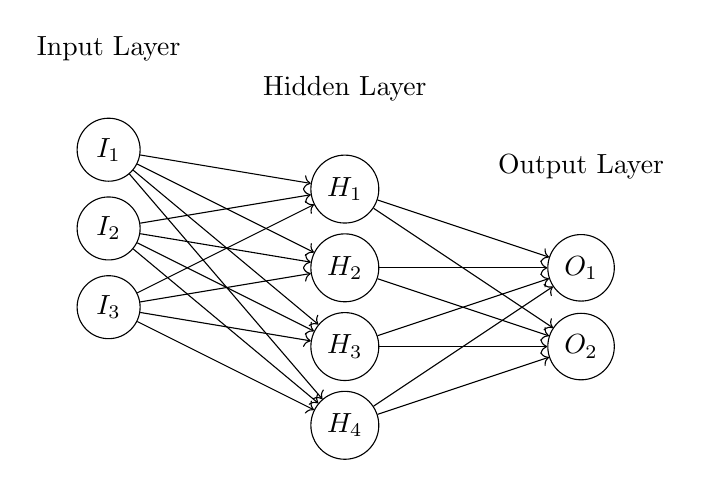
\begin{tikzpicture}[node distance=1.5cm, auto]
    % Input Layer
    \foreach \i in {1,2,3}
        \node[circle, draw, minimum size=0.8cm] (I\i) at (0,-\i) {$I_\i$};
    
    % Hidden Layer
    \foreach \h in {1,2,3,4}
        \node[circle, draw, minimum size=0.8cm] (H\h) at (3, -0.5-\h) {$H_\h$};
        
    % Output Layer
    \foreach \o in {1,2}
        \node[circle, draw, minimum size=0.8cm] (O\o) at (6,-1.5-\o) {$O_\o$};
        
    % Connections
    \foreach \i in {1,2,3}
        \foreach \h in {1,2,3,4}
            \draw [->] (I\i) -- (H\h);
            
    \foreach \h in {1,2,3,4}
        \foreach \o in {1,2}
            \draw [->] (H\h) -- (O\o);
            
    \node[above] at (0,0) {Input Layer};
    \node[above] at (3,-0.5) {Hidden Layer};
    \node[above] at (6,-1.5) {Output Layer};
\end{tikzpicture}
\captionof{figure}{Neural Network Architecture}
\end{center}

\textbf{Information Flow:}
\begin{itemize}
    \item \textbf{Forward Pass}: Input $\to$ Hidden $\to$ Output.
    \item \textbf{Weighted Sum}: $\Sigma(w_i \times x_i + bias)$.
    \item \textbf{Activation}: Apply activation function.
\end{itemize}
\end{solutionbox}

\begin{mnemonicbox}
\mnemonic{IHOC - Input, Hidden, Output, Connections}
\end{mnemonicbox}

\questionmarks{5(c)}{7}{List out and explain types of ambiguities in Natural Language Processing.}
\begin{solutionbox}
\textbf{Ambiguity} in NLP occurs when text has multiple possible interpretations.

\begin{center}
\captionof{table}{Types of NLP Ambiguities}
\begin{tabulary}{\linewidth}{L L L}
\hline
\textbf{Type} & \textbf{Definition} & \textbf{Resolution} \\
\hline
\textbf{Lexical} & Word has multiple meanings & Context analysis \\
\textbf{Syntactic} & Multiple parse structures & Grammar rules \\
\textbf{Semantic} & Multiple sentence meanings & Semantic analysis \\
\textbf{Pragmatic} & Context-dependent meaning & Intent recognition \\
\textbf{Referential} & Unclear pronoun reference & Anaphora resolution \\
\hline
\end{tabulary}
\end{center}

\begin{center}
\begin{tikzpicture}[node distance=1.5cm, auto]
    \node [gtu state] (Ambig) {Ambiguous Text};
    \node [gtu block, right=of Ambig] (Context) {Context Analysis};
    \node [gtu block, right=of Context] (Disambig) {Disambiguation};
    \node [gtu state, right=of Disambig] (Clear) {Clear Interpretation};
    
    \node [gtu block, below=0.5cm of Context] (Knowledge) {Knowledge Bases};
    
    \path [gtu arrow] (Ambig) -- (Context);
    \path [gtu arrow] (Context) -- (Disambig);
    \path [gtu arrow] (Disambig) -- (Clear);
    \path [gtu arrow] (Knowledge) -| (Disambig);
\end{tikzpicture}
\captionof{figure}{Resolution Process}
\end{center}

\textbf{Examples:}
\begin{itemize}
    \item \textbf{Lexical}: "Bank" (river vs financial).
    \item \textbf{Syntactic}: "I saw her duck" (bird vs action).
    \item \textbf{Referential}: "John told Bill he was late" (Who is late?).
\end{itemize}
\end{solutionbox}

\begin{mnemonicbox}
\mnemonic{LSSPR - Lexical, Syntactic, Semantic, Pragmatic, Referential}
\end{mnemonicbox}

\questionmarks{5(a) OR}{3}{List down the names of some popular activation functions used in Neural Network.}
\begin{solutionbox}
\begin{center}
\captionof{table}{Popular Activation Functions}
\begin{tabulary}{\linewidth}{L L L L}
\hline
\textbf{Function} & \textbf{Formula} & \textbf{Range} & \textbf{Usage} \\
\hline
\textbf{ReLU} & \(f(x) = \max(0, x)\) & \([0, \infty)\) & Hidden layers \\
\textbf{Sigmoid} & \(f(x) = 1/(1 + e^{-x})\) & \((0, 1)\) & Binary classification \\
\textbf{Tanh} & \(f(x) = \frac{e^x - e^{-x}}{e^x + e^{-x}}\) & \((-1, 1)\) & Hidden layers \\
\textbf{Softmax} & \(f(x_i) = e^{x_i} / \Sigma e^{x_j}\) & \((0, 1)\) & Multi-class output \\
\hline
\end{tabulary}
\end{center}
\end{solutionbox}

\begin{mnemonicbox}
\mnemonic{RSTSL - ReLU, Sigmoid, Tanh, Softmax, Leaky ReLU}
\end{mnemonicbox}

\questionmarks{5(b) OR}{4}{Explain Learning process in artificial Neural Network.}
\begin{solutionbox}
\textbf{Learning Process} involves adjusting weights and biases to minimize error through iterative training.

\begin{center}
\captionof{table}{Learning Process Steps}
\begin{tabulary}{\linewidth}{L L L}
\hline
\textbf{Step} & \textbf{Process} & \textbf{Description} \\
\hline
\textbf{Initialize} & Random weights & Start with small random values \\
\textbf{Forward Pass} & Calculate output & Propagate input through network \\
\textbf{Calculate Error} & Compare with target & Use loss function \\
\textbf{Backward Pass} & Calculate gradients & Use backpropagation \\
\textbf{Update Weights} & Adjust parameters & Apply gradient descent \\
\hline
\end{tabulary}
\end{center}

\begin{center}
\begin{tikzpicture}[node distance=1.5cm, auto]
    \node [gtu block] (Init) {Initialize Weights};
    \node [gtu block, right=of Init] (Forward) {Forward Pass};
    \node [gtu block, right=of Forward] (Loss) {Calculate Loss};
    \node [gtu block, below=1cm of Loss] (Back) {Backward Pass};
    \node [gtu block, left=of Back] (Update) {Update Weights};
    \node [gtu decision, left=of Update] (Conv) {Converged?};
    \node [gtu state, below=1cm of Conv] (Done) {Training Complete};
    
    \path [gtu arrow] (Init) -- (Forward);
    \path [gtu arrow] (Forward) -- (Loss);
    \path [gtu arrow] (Loss) -- (Back);
    \path [gtu arrow] (Back) -- (Update);
    \path [gtu arrow] (Update) -- (Conv);
    \path [gtu arrow] (Conv) -- node[left] {Yes} (Done);
    \path [gtu arrow] (Conv.north) |- node[left] {No} (Forward.south);
\end{tikzpicture}
\captionof{figure}{Learning Flow}
\end{center}
\end{solutionbox}

\begin{mnemonicbox}
\mnemonic{IFCBU - Initialize, Forward, Calculate, Backward, Update}
\end{mnemonicbox}

\questionmarks{5(c) OR}{7}{List out various advantages and disadvantages of Natural Language Processing.}
\begin{solutionbox}
\begin{center}
\captionof{table}{NLP Advantages and Disadvantages}
\begin{tabulary}{\linewidth}{L L}
\hline
\textbf{Advantages} & \textbf{Disadvantages} \\
\hline
\textbf{Automated Text Analysis} & \textbf{Ambiguity Handling} \\
\textbf{Language Translation} & \textbf{Context Understanding} \\
\textbf{Human-Computer Interaction} & \textbf{Cultural Nuances} \\
\textbf{Information Extraction} & \textbf{Computational Complexity} \\
\textbf{Sentiment Analysis} & \textbf{Data Requirements} \\
\hline
\end{tabulary}
\end{center}

\begin{center}
\begin{tikzpicture}[node distance=1.5cm]
    \node [gtu block] (NLP) {NLP};
    
    \node [gtu state, below left=1.5cm and 0.5cm of NLP, align=center] (Apps) {\textbf{Applications}\\Translation\\Sentiment\\Extraction};
    \node [gtu state, below right=1.5cm and 0.5cm of NLP, align=center] (Challenges) {\textbf{Challenges}\\Ambiguity\\Context\\Nuances};
    
    \path [gtu arrow] (NLP) -- (Apps);
    \path [gtu arrow] (NLP) -- (Challenges);
\end{tikzpicture}
\captionof{figure}{Applications vs Challenges}
\end{center}

\textbf{Advantages:}
\begin{itemize}
    \item \textbf{Business}: Customer service chatbots, content analysis.
    \item \textbf{Technical}: Scalability, consistency, speed.
\end{itemize}

\textbf{Disadvantages:}
\begin{itemize}
    \item \textbf{Challenges}: Ambiguity, sarcasm detection, domain specificity.
    \item \textbf{Resources}: Requires large datasets and computational power.
\end{itemize}
\end{solutionbox}

\begin{mnemonicbox}
\mnemonic{ALICE vs ACHDR - Automated, Language, Interaction, Content, Extraction vs Ambiguity, Context, Human-nuances}
\end{mnemonicbox}

\end{document}
